\documentclass{article}

\usepackage[top=1in,left=1.5in,right=1.5in,bottom=1.5in]{geometry}

\usepackage{pgfplots}
\usetikzlibrary{angles, arrows.meta, calc, quotes}
\pgfplotsset{width=0.8\textwidth,compat=1.18}

\usepackage{subcaption}

\usepackage{booktabs}

\usepackage{graphicx}
\let\rfb\reflectbox
\graphicspath{ {images} }

\usepackage{cancel}

\usepackage{mathtools}

\usepackage{nicefrac}
\newcommand{\flippedfrac}[2]{\rfb{\nicefrac{\rfb{#2}}{\rfb{#1}}}}



\usepackage{amsthm}
\renewcommand{\qedsymbol}{$\blacksquare$}
\usepackage{amssymb}
\usepackage{amsmath}
\newcommand\numberthis{\addtocounter{equation}{1}\tag{\theequation}}
\DeclareMathOperator*{\argmax}{arg\,max}
\DeclareMathOperator*{\argmin}{arg\,min}

\usepackage{hyperref}
\hypersetup{
    colorlinks = true,
}


\usepackage{titling}
\title{Exercise Set 4 - Reinforcement Learning}
\newcommand{\subtitle}[1]{%
  \posttitle{%
    \par\end{center}
    \begin{center}\large#1\end{center}
    \vskip0.5em}%
}
\makeatother
\subtitle{Control with approximation and policy gradients}
\author{Giulio Starace - 13010840}
\date{\today}

\begin{document}
\maketitle
\section*{Homework: Geometry of linear value-function approximation (Application)}
\begin{enumerate}
	\item \label{q:7.4.1} To compute the Bellman error vector after initialization, we compute the
	      Bellman error for each state. We first recall the definition of the Bellman operator $B^\pi$:
	      \begin{equation}
		      (B^\pi v)(s) ~ \dot{=} ~ \sum_a \pi(a | s) \sum_{s', r} p(s', r | s, a) \left[ r + \gamma
			      v(s') \right].
	      \end{equation}
	      We can plug this into the definition of the Bellman error:
	      \begin{align*}
		      \overline{\delta}_w(s) & = B^\pi v_w - v_w                                       \\
		                             & = \sum_a \pi(a | s) \sum_{s', r} p(s', r | s, a) \left[
			      r + \gamma v_w(s') \right] - v_w(s).
	      \end{align*}
	      For $s_0$, we have a single action available that is always taken, so our $\sum_a
		      \pi(a | s)$ term disappears and we are left with:
	      \begin{equation}
		      \overline{\delta}_w(s) = \sum_{s', r} p(s', r | s) \left[r + \gamma
			      v_w(s') \right] - v_w(s)
	      \end{equation}
	      Our action always leads to the same state, with the same reward (of 0), so we can simplify further
	      and write
	      \begin{equation}
		      \overline{\delta}_w(s) = \gamma v_w(s') - v_w(s).
	      \end{equation}
	      Finally, we have that $v_{w, s} = w \cdot \phi_s$, so that we can write
	      \begin{equation}
		      \overline{\delta}_w(s) = \gamma w \cdot \phi_{s'} - w \cdot \phi_s.
	      \end{equation}
	      The same arguments can be applied to $s_1$, so we can write the Bellman error
	      \textit{vector} as
	      \begin{equation}
		      \text{BE}(w) = \left(\overline{\delta}_w(s_0), ~ \overline{\delta}_w(s_1) \right)^T = \left(
		      \gamma w \cdot \phi_{s_1} - w \cdot \phi_{s_0}, ~ \gamma w \cdot \phi_{s_0} - w
		      \cdot \phi_{s_1} \right)^T.
	      \end{equation}
	      We can plug in our values $w =1$, $\phi_{s_0} = 2$, $\phi_{s_1} = 1$, and $\gamma =1$ and
	      obtain
	      \begin{equation}
		      \text{BE}(w) = \left(1 \cdot1 - 1 \cdot 2, ~ 1 \cdot 2 - 1 \cdot 1\right)^T = \left(-1, ~ 1\right)^T.
	      \end{equation}
	\item The Mean Squared Bellman Error $\overline{\text{BE}}(w)$ is the measure of the overall error in the
	      value function, computed by taking the $\mu$ weighted norm of the Bellman error vector. Here,
	      $\mu$ is a distribution $\mu : \mathcal{S} \rightarrow \left[0, 1\right]$ specifying the extent
	      to which each state is considered in the computation. Mathematically:
	      \begin{equation}
		      \overline{\text{BE}}(w) = \lVert \text{BE}(w) \rVert^2_\mu = \sum_s \mu(s) \overline{\delta}_w(s)^2.
	      \end{equation}
	      In our case, this would be expressed as
	      \begin{equation}
		      \overline{\text{BE}}(w) = \mu(s_0) \cdot (-1)^2 + \mu(s_1) \cdot 1^2 = \mu(s_0) + \mu(s_1)
		      = \sum_s \mu(s).
	      \end{equation}
	\item The target values $B^\pi v_w$ we found in question \ref{q:7.4.1}. are 1 for $s_0$ and 2 for
	      $s_1$. The $w$ that results in the value function that is closest can be applied using
	      a least-squares regression:
	      \begin{align*}
		      \beta & = \argmin_\beta  \lVert \mathbf{Y} - w \mathbf{X} \rVert^2               \\
		      w     & = \argmin_w  \lVert (1, ~2 )^T - w (\phi_{s_0}, ~ \phi_{s_1})^T \rVert^2 \\
		            & = \argmin_w\lVert (1, ~2 )^T - w (2, 1)^T \rVert^2. \numberthis
	      \end{align*}
	      This has a closed-form solution:
	      \begin{equation}
		      \beta = \left(\mathbf{X}^T \mathbf{X}\right)^{-1} \mathbf{X}^T \mathbf{Y},
	      \end{equation}
	      which for our numbers gives $w = 4/5$.
	\item The plot of $v_w$, $B^\pi v_w$ and $\Pi B^\pi v_w$ is shown in Figure \ref{fig:7.4.4}. TODO
	      % put image here		
	      \begin{figure}[ht!]
		      \centering
		      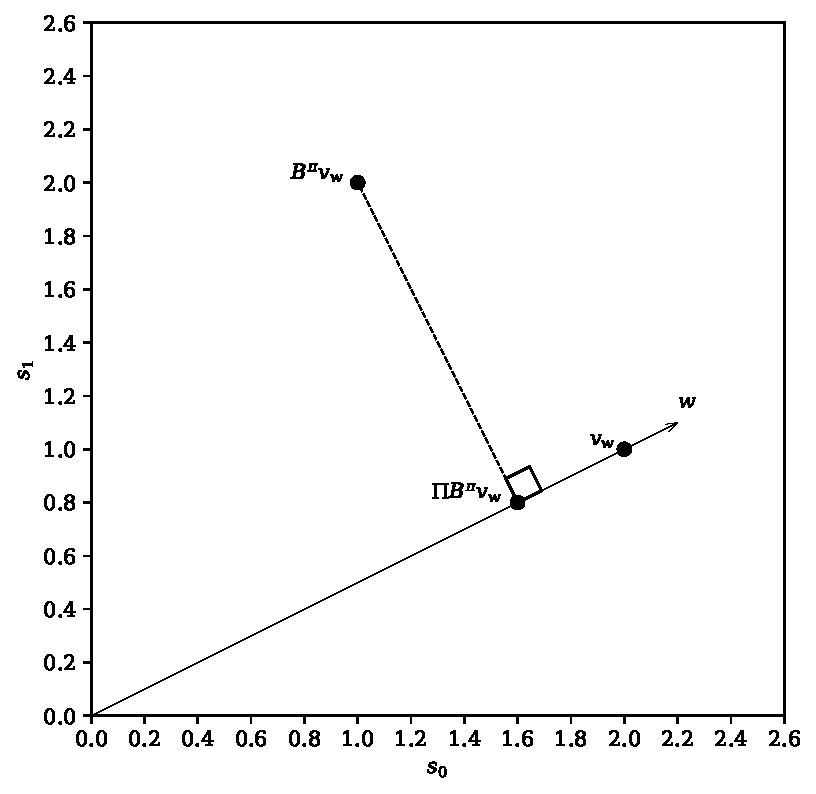
\includegraphics[width=0.8\textwidth]{images/7.4.4.pdf}
		      \caption{TODO}
		      \label{fig:7.4.4}
	      \end{figure}

\end{enumerate}
\section*{Homework: Coding Assignment - Deep Q Networks}
\begin{enumerate}
	\item Coding answers have been submitted on codegra under the group ``stalwart cocky sawly".
	\item hello world
\end{enumerate}

\section*{Homework: REINFORCE}
\begin{enumerate}
	\item The update to the policy parameter  $\theta$ under classical REINFORCE is given by
	      \begin{equation}
		      \theta_{t+1} \leftarrow \theta_t + \alpha \bighat{\nabla J}
	      \end{equation}
	\item hello world
	\item hello world
	\item hello world
	\item hello world
\end{enumerate}


\end{document}

